\documentclass[aspectratio=169,11pt]{ctexbeamer}

\usetheme{Madrid}
\usecolortheme{seahorse}
\usefonttheme{professionalfonts}
\setbeamertemplate{navigation symbols}{}
\setbeamertemplate{caption}[numbered]

\usepackage{booktabs}
\usepackage{tabularx}
\usepackage{array}
\usepackage{graphicx}
\usepackage{multirow}
\usepackage{arydshln}
\usepackage{colortbl}
\usepackage{tikz}
\usepackage{amsmath}
\usepackage{amssymb}
\usepackage{mathtools}

\usetikzlibrary{arrows.meta,positioning,shapes.geometric,fit}

\definecolor{MainBlue}{RGB}{33,92,135}
\definecolor{SoftBlue}{RGB}{229,240,248}
\definecolor{AccentGreen}{RGB}{49,128,97}
\definecolor{AccentRed}{RGB}{172,73,68}
\definecolor{DarkGray}{RGB}{65,70,75}


\setbeamercolor{title}{fg=MainBlue}
\setbeamercolor{frametitle}{fg=MainBlue}
\setbeamercolor{structure}{fg=MainBlue}
\setbeamercolor{block title}{bg=MainBlue,fg=white}
\setbeamercolor{block body}{bg=SoftBlue,fg=black}

\newcommand{\code}[1]{\texttt{\small\detokenize{#1}}}
\newcommand{\ok}{\textcolor{AccentGreen}{\(\checkmark\)}}
\newcommand{\warn}{\textcolor{AccentRed}{\(\triangle\)}}
\DeclareMathOperator{\Tr}{Tr}
\DeclareMathOperator{\mean}{mean}
\DeclareMathOperator{\diag}{diag}
\newcommand{\ind}{\mathbf{1}}

\title[Quant-dLLM 复现流程]{Reproduction of Quant-dllm}
\author[czh]{czh}
\date{\today}

\begin{document}

\begin{frame}
  \titlepage
\end{frame}

\begin{frame}{演示目标}
  \begin{itemize}
    \item 复现对象：Quant-dLLM 在 LLaDA-8B-Base 上的 2-bit weight-only PTQ。
    \item 当前主线：column-group DAQ/ABMP + DOR + GPTQ/OBC-style compensation。
    \item 主要入口：\code{tools/quant_stagewise_pipeline.py} 和 \code{scripts/local_stagewise_quant_eval.sh}。
    \item 验证目标：WinoGrande 从早期复现的 0.6267 提升到当前主线的 0.6614。
  \end{itemize}
\end{frame}

\begin{frame}{项目结构}
  \footnotesize
  \begin{columns}[T]
    \begin{column}{0.49\linewidth}
      \begin{block}{算法模块}
        \begin{itemize}
          \item \code{MCS/load_dataset.py}\\
          构造 C4 校准样本和 timestep mask states。
          \item \code{utils/generate_imp_mat.py}\\
          收集 SMCS，构造 \(Z\)，处理 inverse diagonal。
          \item \code{DAQ/quantizer.py}\\
          实现 RSR、DOR mask 和 binary pattern search。
          \item \code{ABMP/allocator.py}\\
          保留早期接口；主线分配逻辑在 \code{main.py}。
        \end{itemize}
      \end{block}
    \end{column}
    \begin{column}{0.49\linewidth}
      \begin{block}{流程与文档}
        \begin{itemize}
          \item \code{tools/quant_stagewise}\\
          \code{_pipeline.py}\\
          分 block、分 stage 收集统计并写回量化权重。
          \item \code{scripts/local_stagewise}\\
          \code{_quant_eval.sh}\\
          包装量化、模型保存和 LLaDA benchmark。
          \item \code{docs/stagewise_gptq}\\
          \code{_daq_quantization.md}\\
          记录当前最对齐论文的公式、配置和结果。
        \end{itemize}
      \end{block}
    \end{column}
  \end{columns}
\end{frame}

\begin{frame}{复现流程}
  \centering
  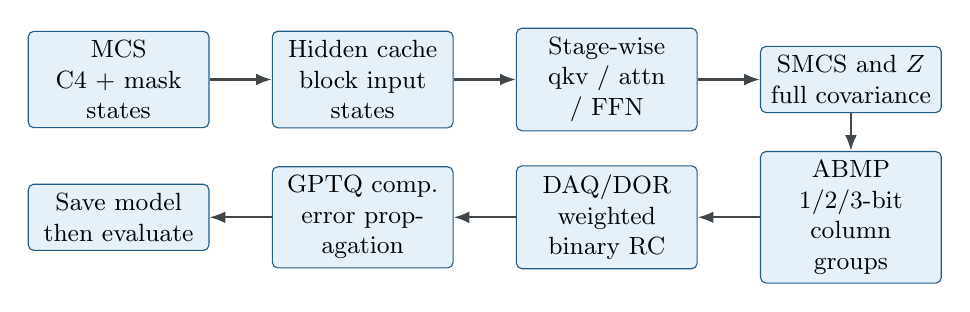
\begin{tikzpicture}[
    flowstep/.style={draw=MainBlue, rounded corners=2pt, fill=SoftBlue, text width=0.17\linewidth, align=center, minimum height=0.82cm, font=\small},
    arrow/.style={-{Latex[length=2.0mm]}, thick, draw=DarkGray}
  ]
    \node[flowstep] (mcs) at (0,0) {MCS\\C4 + mask states};
    \node[flowstep] (hidden) at (3.1,0) {Hidden cache\\block input states};
    \node[flowstep] (stage) at (6.2,0) {Stage-wise\\qkv / attn / FFN};
    \node[flowstep] (smcs) at (9.3,0) {SMCS and \(Z\)\\full covariance};
    \node[flowstep] (abmp) at (9.3,-1.75) {ABMP\\1/2/3-bit column groups};
    \node[flowstep] (daq) at (6.2,-1.75) {DAQ/DOR\\weighted binary RC};
    \node[flowstep] (gptq) at (3.1,-1.75) {GPTQ comp.\\error propagation};
    \node[flowstep] (eval) at (0,-1.75) {Save model\\then evaluate};

    \draw[arrow] (mcs.east) -- (hidden.west);
    \draw[arrow] (hidden.east) -- (stage.west);
    \draw[arrow] (stage.east) -- (smcs.west);
    \draw[arrow] (smcs.south) -- (abmp.north);
    \draw[arrow] (abmp.west) -- (daq.east);
    \draw[arrow] (daq.west) -- (gptq.east);
    \draw[arrow] (gptq.west) -- (eval.east);
  \end{tikzpicture}

  \vspace{0.4cm}
  \small
  每个 stage 的统计Z cache来自当前已经部分量化的模型状态。
\end{frame}

\begin{frame}{论文流程}
  \small
  \begin{block}{主线逻辑}
    Diffusion LLM 的 mask/time-step 激活分布不同于 AR LLM，因此传统 GPTQ 类 PTQ 在 W2A16/W3A16 下会明显退化；引入 binarization、MCS、DAQ/DOR 和 ABMP。
  \end{block}

  \begin{columns}[T]
    \begin{column}{0.48\linewidth}
      \begin{enumerate}
        \item MCS 构造 timestep-aware masked calibration set。
        \item 逐个 Linear 层收集输入激活，计算 importance matrix \(Z\)。
        \item ABMP 根据 \(Z\) 对 column block 分配 1/2/3 bit。
      \end{enumerate}
    \end{column}
    \begin{column}{0.48\linewidth}
      \begin{enumerate}
        \setcounter{enumi}{3}
        \item DAQ 用多阶 1-bit 分量叠加近似 K-bit 权重。
        \item DOR 对 \(Z\)-outlier 提高重构权重。
        \item 量化目标层后进入评测和消融对齐。
      \end{enumerate}
    \end{column}
  \end{columns}

  \vspace{0.18cm}
  \footnotesize
  MCS \(\rightarrow\) layer-by-layer ( \(Z\) \(\rightarrow\) ABMP \(\rightarrow\) DAQ )
\end{frame}

\begin{frame}{复现流程}
  \centering
  \begin{tikzpicture}[
    pstep/.style={draw=MainBlue, fill=SoftBlue, rounded corners=2pt, text width=0.15\linewidth, align=center, minimum height=0.76cm, font=\scriptsize},
    varrow/.style={-{Latex[length=1.8mm]}, thick, draw=DarkGray}
  ]
    \node[pstep] (cfg) at (0,0) {固定配置};
    \node[pstep] (calib) at (2.75,0) {C4 数据集校准\\MCS states};
    \node[pstep] (hook) at (5.5,0) {stage hooks\\收集 \(X^\top X\)};
    \node[pstep] (z) at (8.25,0) {SMCS inverse\\构造 \(Z\)};
    \node[pstep] (alloc) at (11,0) {ABMP\\column groups};
    \node[pstep] (quant) at (11,-1.62) {DAQ/DOR\\写回 stage};
    \node[pstep] (comp) at (8.25,-1.62) {GPTQ comp.\\补偿后续列};
    \node[pstep] (cache) at (5.5,-1.62) {传播 hidden\\进入下一 stage};
    \node[pstep] (save) at (2.75,-1.62) {保存 HF\\fake-quant ckpt};
    \node[pstep] (eval) at (0,-1.62) {Benchmark\\任务对齐};

    \draw[varrow] (cfg.east) -- (calib.west);
    \draw[varrow] (calib.east) -- (hook.west);
    \draw[varrow] (hook.east) -- (z.west);
    \draw[varrow] (z.east) -- (alloc.west);
    \draw[varrow] (alloc.south) -- (quant.north);
    \draw[varrow] (quant.west) -- (comp.east);
    \draw[varrow] (comp.west) -- (cache.east);
    \draw[varrow] (cache.west) -- (save.east);
    \draw[varrow] (save.west) -- (eval.east);
    \draw[varrow, dashed] (cache.north) -- (hook.south);
  \end{tikzpicture}

  \vspace{0.25cm}
  \small
  ``layer-by-layer'' 进一步细化为 block 内四个 stage：\code{qkv}、\code{attn_out}、\code{ff_in}、\code{ff_out}。每个 stage 量化后立即写回，因此后续统计看到的是当前量化状态。
\end{frame}

\begin{frame}{从复现到定位问题的实验闭环}
  \small
  \begin{columns}[T]
    \begin{column}{0.31\linewidth}
      \begin{block}{1. 对齐配置}
        \begin{itemize}
          \item 固定 \code{nsamples=128}
          \item 固定 \code{seqlen=4096}
          \item 固定 \code{block/group=128}
        \end{itemize}
      \end{block}
    \end{column}
    \begin{column}{0.31\linewidth}
      \begin{block}{2. 对齐链路}
        \begin{itemize}
          \item 先复测 FP baseline
          \item 再测 GPTQ/GPTAQ/Slim-LLM
          \item 最后测 Quant-dLLM
          \item 只用 full benchmark 做论文对比
        \end{itemize}
      \end{block}
    \end{column}
    \begin{column}{0.31\linewidth}
      \begin{block}{3. 定位差距}
        \begin{itemize}
          \item 看 \(Z\)-weighted error
          \item 看 bit allocation map
          \item 消融 granularity / damping
        \end{itemize}
      \end{block}
    \end{column}
  \end{columns}

  \vspace{0.2cm}
  \begin{block}{当前判断}
    复现主线已经把之前 0.61--0.63 的 WinoGrande 恢复到 0.6614；剩余差距更像是 FP 评测链路、任务细节和论文未公开超参共同造成，因为 FP 模型的评测精度也会比论文略低 1-2 个百分点
  \end{block}
\end{frame}

\begin{frame}{当前主线配置}
  \small
  \begin{columns}[T]
    \begin{column}{0.49\linewidth}
      \begin{block}{校准与 SMCS}
        \begin{itemize}
          \item \code{nsamples=128}, \code{seqlen=4096}
          \item \code{num_steps=20}, linear schedule
          \item \code{mcs_no_full_visible=true}
          \item \code{mcs_normalization=tokens}
          \item \code{max_tokens_per_state=0}
          \item \code{damping_mode=diag_mean}
          \item \code{damp_percent=0.01}
        \end{itemize}
      \end{block}
    \end{column}
    \begin{column}{0.49\linewidth}
      \begin{block}{量化与分配}
        \begin{itemize}
          \item \code{daq_granularity=column}
          \item \code{abmp_granularity=column}
          \item \code{abmp_rank_scope=weight}
          \item \code{quant_block_size=128}
          \item \code{allocate_ratio=0.05}
          \item \code{daq_component=rsr_w_dor}
          \item \code{gptq_compensation=1}
        \end{itemize}
      \end{block}
    \end{column}
  \end{columns}
\end{frame}

\begin{frame}{MCS 对齐 dLLM 的可见性分布}
  \begin{block}{代码位置}
    \code{MCS/load_dataset.py} 负责 C4 采样、mask token 查询、timestep grid 和 Bernoulli visibility。
  \end{block}

  \begin{itemize}
    \item 每条 C4 序列长度固定为 4096，校准样本数固定为 128。
    \item 前缀比例 \(\gamma=0.25\)：前缀始终可见，后续 token 由 timestep 的 \(\alpha(t)\) 控制。
    \item \code{mcs_no_full_visible} 去掉完全可见 endpoint，避免校准统计偏向普通 AR 输入。
    \item 生成的 calibration states 进入 stage-wise pipeline，后续 hooks 收集每个 Linear 的 \(X^\top X\)。
  \end{itemize}
\end{frame}

\begin{frame}{Stage-wise pipeline 让统计跟随量化状态}
  \small
  \begin{columns}[T]
    \begin{column}{0.45\linewidth}
      \begin{block}{每个 transformer block 内的顺序}
        \begin{enumerate}
          \item \code{qkv}: \code{q_proj}, \code{k_proj}, \code{v_proj}
          \item \code{attn_out}: \code{attn_out}
          \item \code{ff_in}: \code{ff_proj}, \code{up_proj}
          \item \code{ff_out}: \code{ff_out}
        \end{enumerate}
      \end{block}
    \end{column}
    \begin{column}{0.53\linewidth}
      \begin{itemize}
        \item 对当前 stage 注册 hooks，只收集该 stage 的输入统计。
        \item 量化后立即写回 in-memory model。
        \item 后续 stage 看到的是已经量化过的上游模块。
        \item block 完成后，传播完整量化 block 输出作为下一层 hidden cache。
      \end{itemize}
    \end{column}
  \end{columns}
\end{frame}

\begin{frame}{SMCS 与 \(Z\) 构造是 DOR 和 ABMP 的共同来源}
  \begin{block}{输出优化目标}
    \[
      \left\lVert XW^\top - XQ^\top \right\rVert_F^2
      =
      \Tr\bigl((W-Q)S(W-Q)^\top\bigr),
      \quad S = X^\top X / N.
    \]
  \end{block}

  \begin{block}{论文实现的 \(Z\)}
    \[
      \epsilon = 0.01 \cdot \mean(\diag(S)),\quad
      H=(S+\epsilon I)^{-1},\quad
      Z_{ij}=\left(\frac{W_{ij}}{\max(\diag(H)_j,\tau)}\right)^2.
    \]
  \end{block}

  \small
  \(Z\) 同时决定 ABMP 的 block score 和 DAQ/DOR 的 outlier mask。
\end{frame}

\begin{frame}{ABMP 在每个 Linear 内重分配 column-group bit-width}
  \begin{block}{分组}
    \[
      G_k = W[:, 128k : 128(k+1)],
      \qquad
      s(G_k)=\sum_{(i,j)\in G_k} Z_{ij}.
    \]
  \end{block}

  \begin{itemize}
    \item \code{abmp_rank_scope=weight}：每个 Linear 只和自己的 column groups 排序。
    \item \code{allocate_ratio=0.05}：最低 5\% 分到 1 bit，最高 5\% 分到 3 bit。
    \item 中间 groups 保持 2 bit，使每个权重矩阵平均 bit-width 接近 2。
    \item column group 与 GPTQ compensation 的顺序更新天然匹配。
  \end{itemize}
\end{frame}

\begin{frame}{DAQ/DOR 把重要性压缩成可解的加权 Frobenius 目标}
  \begin{block}{DOR mask}
    \[
      \Pi_{ij}=\ind\{|Z_{ij}-\mu(Z_\mathrm{unit})| > 3\sigma(Z_\mathrm{unit})\},
      \qquad
      \Lambda_{ij}=1+(\lambda-1)\Pi_{ij}.
    \]
  \end{block}

  \begin{block}{DAQ 表示}
    \[
      Q=\sum_{t=1}^{b}
      \left(\alpha_r^{(t)}(\alpha_c^{(t)})^\top\right)\odot B^{(t)},
      \quad B^{(t)}\in\{-1,+1\}^{\text{rows}\times\text{cols}}.
    \]
  \end{block}

  \small
  \code{DAQ/quantizer.py} 通过 closed-form scale updates 和 \(2^b\) pattern search 交替优化。
\end{frame}

\begin{frame}{GPTQ/OBC-style compensation}
  论文并没有显式提到做 GPTQ style compensation，但缺乏该优化的 pipeline 评测效果离论文有一定差距，通过查阅论文引用的 ARB-LLM 和 Bi-LLM，其中均有提到工程实现用类似 GPTQ 的 block-wise compensation 进行改造，这一优化很可能是默认的工程实现
  \begin{block}{按列组顺序修正后续残差}
    对 column group \(c_s:c_e\) 量化后，当前实现用 inverse Cholesky factor \(U\) 更新后续列：
    \[
      E=(W_\mathrm{work}[:,c_s:c_e]-Q[:,c_s:c_e])/\diag(U_\mathrm{block}),
    \]
    \[
      W_\mathrm{work}[:,c_e:]=W_\mathrm{work}[:,c_e:] - E U_\mathrm{cross}.
    \]
  \end{block}

  \begin{itemize}
    \item 该路径要求 \code{daq_granularity=column}。
    \item 它使用 full-SMCS inverse factor，不适合旧的 blockdiag \(Z\) cache。
    \item 这是早期 baseline 到当前主线提升的主要实现差异。
  \end{itemize}
\end{frame}

\begin{frame}{主入口与工具脚本的分工}
  \small
  \begin{tabularx}{\linewidth}{>{\raggedright\arraybackslash}p{0.32\linewidth}X}
    \toprule
    文件 & 使用场景 \\
    \midrule
    \code{main.py} & 通用离线量化入口；支持 \(Z\) cache、ABMP、DAQ、row/tile/column ablations。 \\
    \code{tools/quant_stagewise_pipeline.py} & 当前最强主线；stage-wise 统计、量化写回、GPTQ compensation。 \\
    \code{tools/quant_layerwise_pipeline.py} & layer-wise 复现路径；用于对照论文的 layer-wise 描述。 \\
    \code{tools/build_full_smcs_z_cache.py} & full-SMCS \(Z\) cache 构造；用于诊断或非主线实验。 \\
    \code{tools/diagnose_full_smcs.py} & full-SMCS 与 blockdiag \(Z\) 的一致性诊断。 \\
    \code{tools/diagnose_quant_alignment.py} & precision map、mask 覆盖率、重构误差和 \(Z\)-weighted error 诊断。 \\
    \bottomrule
  \end{tabularx}
\end{frame}

\begin{frame}{主线和消融分开运行}
  \small
  \begin{itemize}
    \item \code{scripts/local_stagewise_quant_eval.sh}：当前主线入口，量化后可直接运行 benchmark。
    \item \code{scripts/exp_quantdllm_ablation_quantize.sh}：ABMP ratio、calibration size、granularity 消融。
    \item \code{scripts/exp_quantdllm_ablation_eval_mmlu.sh}：批量评测量化模型的 MMLU。
    \item \code{scripts/exp_gptq_llada8b_baseline.sh}：调用 QDLM/AutoGPTQ 作为 baseline。
    \item \code{scripts/exp_cross_model_template.sh}：Dream 或其他 LLaDA 变体的迁移模板。
    \item \code{llada_benchmark.sh}：评测封装，复用 QDLM 风格的任务和 Monte Carlo 设置。
  \end{itemize}
\end{frame}

\begin{frame}[fragile]{可复现主线命令}
  \scriptsize
  \begin{verbatim}
RUN_ID=stagewise_gptq_comp_colabmp_n128_s4096_t20_tok0_diag1p_$(date +%Y%m%d_%H%M%S) \
CUDA_VISIBLE_DEVICES=0,1,2 \
PYTHON_BIN=/root/miniconda3/envs/qdlm/bin/python \
C4_SOURCE=/root/data-fs/c4-train/c4-train.00000-of-01024.json.gz \
MAX_TOKENS_PER_STATE=0 \
DAMPING=0.0 DAMPING_MODE=diag_mean DAMP_PERCENT=0.01 \
DAQ_GRANULARITY=column ABMP_GRANULARITY=column ABMP_RANK_SCOPE=weight \
QUANT_BLOCK_SIZE=128 ALLOCATE_RATIO=0.05 DEFAULT_BITS=2 \
DAQ_STEPS=10 IMP_LAMDA=2.0 DOR_MASK_SCOPE=unit \
DAQ_COMPONENT=rsr_w_dor GPTQ_COMPENSATION=1 DAQ_FULLS_REFINE=0 \
RUN_EVAL=1 EVAL_TASKS=winogrande EVAL_LIMIT=full \
bash scripts/local_stagewise_quant_eval.sh
  \end{verbatim}

  \normalsize
  \begin{block}{执行约束}
    \code{EVAL_LIMIT=full} 才能和论文表格对比；\code{EVAL_LIMIT=200} 只用于 smoke test。
  \end{block}
\end{frame}

\begin{frame}{输出目录}
  \small
  \begin{columns}[T]
    \begin{column}{0.48\linewidth}
      \begin{block}{量化产物}
        \begin{itemize}
          \item \code{outputs/<run_id>/}
          \item \code{stagewise_args.json}
          \item \code{precision_map.json}
          \item \code{importance_scores.json}
          \item \code{quantized_blocks/*.safetensors}
          \item 重写后的 HF checkpoint
        \end{itemize}
      \end{block}
    \end{column}
    \begin{column}{0.48\linewidth}
      \begin{block}{诊断产物}
        \begin{itemize}
          \item \code{z_cache/block_XX.safetensors}
          \item inverse report
          \item hidden cache
          \item benchmark results
          \item run logs and pid files
        \end{itemize}
      \end{block}
    \end{column}
  \end{columns}
\end{frame}

\begin{frame}{非主线变体}
  \small
  \begin{tabularx}{\linewidth}{>{\raggedright\arraybackslash}p{0.34\linewidth}X}
    \toprule
    变体 & 用途 \\
    \midrule
    \code{daq_fulls_refine} & 固定 \(B\) 后用 full-S Hessian 细化 scales；当前不是解释 WinoGrande 提升的必要项。 \\
    \code{daq_activation_diag} & 使用 activation diagonal 作为求解权重；属于 activation-aware DAQ 诊断。 \\
    \code{daq_row_center} / \code{daq_block_row_center} & row-centering 消融；当前主线关闭。 \\
    \code{tile} / \code{row} / \code{weight} granularity & 分块方式消融；当前主线使用 column groups。 \\
    \code{full-SMCS Z cache} & 诊断 full covariance 和 blockdiag 近似差异，不作为 stage-wise 主线缓存复用。 \\
    \bottomrule
  \end{tabularx}
\end{frame}

\begin{frame}{论文报告的 LLaDA-8B-Base 目标结果}
  \scriptsize
  \centering
  \renewcommand{\arraystretch}{1.25}
  \resizebox{\linewidth}{!}{
    \begin{tabular}{l | l | c c c c c c c | c}
      \toprule
      \rowcolor{black!5}
      \textbf{Model} & \textbf{Method}
      & \textbf{MMLU(5)} & \textbf{Wino.(5)} & \textbf{PIQA(0)}
      & \textbf{ARC-C(0)} & \textbf{ARC-E(0)} & \textbf{Hella.(0)}
      & \textbf{BBH(0)} & \textbf{Avg} \\
      \midrule
      \multirow{5}{*}{\textbf{LLaDA-8B-Base}}
      & FP
      & 65.76 & 74.59 & 74.70 & 44.11 & 74.20 & 54.27 & 42.60 & 61.46 \\
      \cdashline{2-10}
      & GPTQ
      & 34.75 & 57.85 & 57.45 & 22.44 & 37.04 & 33.77 & 4.06 & 35.34 \\
      & GPTAQ
      & 34.73 & 59.04 & 56.42 & 22.27 & 38.17 & 35.13 & 5.34 & 35.87 \\
      & Slim-LLM
      & 47.98 & 60.85 & 62.46 & 26.11 & 53.41 & 39.25 & 6.64 & 42.39 \\
      & \textbf{Quant-dLLM}
      & \textbf{56.87} & \textbf{68.19} & \textbf{69.75}
      & \textbf{36.26} & \textbf{68.69} & \textbf{46.45}
      & \textbf{32.18} & \textbf{54.06} \\
      \bottomrule
    \end{tabular}
  }

  \vspace{0.25cm}
  \small
  原论文在 7 个任务上报告 Quant-dLLM 平均 54.06，其中 WinoGrande 为 68.19，BBH 为 32.18。
\end{frame}

\begin{frame}{本次复现结果汇总}
  \scriptsize
  \centering
  \resizebox{\linewidth}{!}{
    \begin{tabular}{l l c c c c c c c c}
      \toprule
      Model & Method & MMLU(5) & Wino.(5) & PIQA(0) & ARC-C(0) & ARC-E(0) & Hella.(0) & BBH(0) & Avg \\
      \midrule
      LLaDA-8B-Base & FP & --- & 73.40 & 72.25 & 41.81 & 73.40 & --- & 40.70 & 60.31 \\
      \midrule
      LLaDA-8B-Base & GPTQ & 34.75 & 57.85 & 57.45 & 22.44 & 37.04 & 33.77 & 4.06 & 35.34 \\
      LLaDA-8B-Base & GPTAQ & 34.73 & 59.04 & 56.42 & 22.27 & 38.17 & 35.13 & 5.34 & 35.87 \\
      LLaDA-8B-Base & Slim-LLM & 47.98 & 60.85 & 62.46 & 26.11 & 53.41 & 39.25 & 6.64 & 42.39 \\
      LLaDA-8B-Base & \textbf{Quant-dLLM} & \textbf{---} & \textbf{66.14} & \textbf{65.67} & \textbf{34.90} & \textbf{67.13} & \textbf{---} & \textbf{28.47} & \textbf{52.46} \\
      \bottomrule
    \end{tabular}
  }

  \vspace{0.25cm}
  \begin{block}{口径说明}
    \small
    由于时间问题，复现 Quant-dLLM 缺少 MMLU 和 HellaSwag，Avg 只统计 WinoGrande、PIQA、ARC-C、ARC-E、BBH 五个共同任务。
  \end{block}
\end{frame}

\begin{frame}{同任务对齐后的差距分析}
  \scriptsize
  \centering
  \begin{tabular}{l c c c c}
    \toprule
    Task & Paper Quant & Reproduced Quant & Gap & Local FP retention \\
    \midrule
    WinoGrande & 68.19 & 66.14 & -2.05 & 90.1\% \\
    PIQA & 69.75 & 65.67 & -4.08 & 90.9\% \\
    ARC-C & 36.26 & 34.90 & -1.36 & 83.5\% \\
    ARC-E & 68.69 & 67.13 & -1.56 & 91.5\% \\
    BBH & 32.18 & 28.47 & -3.71 & 70.0\% \\
    \midrule
    Common-task Avg & 55.01 & 52.46 & -2.55 & 87.0\% \\
    \bottomrule
  \end{tabular}

  \vspace{0.35cm}
  \begin{itemize}
    \item 绝对差距为 2.55 \%，但本地 FP 在五个共同任务上也比论文 FP 低 1.73 \%。
    \item 考虑 FP 链路差异，可以说明主线已经接近论文结果。
    \item 主要差异来自 PIQA 和 BBH；ARC-C 与 ARC-E 的相对对齐更好。
  \end{itemize}
\end{frame}

\begin{frame}{附录：模块依赖图}
  \centering
  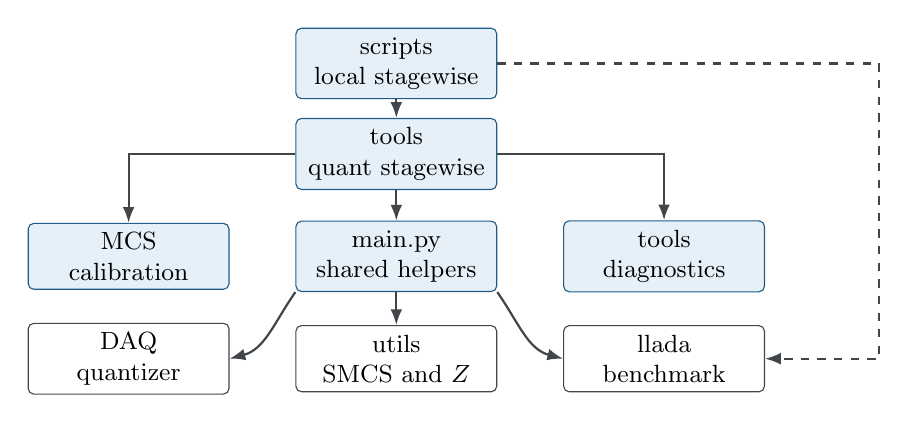
\begin{tikzpicture}[
    mod/.style={draw=MainBlue, fill=SoftBlue, rounded corners=2pt, align=center, minimum width=2.55cm, minimum height=0.72cm, font=\small},
    aux/.style={draw=DarkGray, fill=white, rounded corners=2pt, align=center, minimum width=2.55cm, minimum height=0.72cm, font=\small},
    arrow/.style={-{Latex[length=2mm]}, thick, draw=DarkGray}
  ]
    \node[mod] (script) at (0,0) {scripts\\local stagewise};
    \node[mod] (tool) at (0,-1.15) {tools\\quant stagewise};
    \node[mod] (mcs) at (-3.4,-2.45) {MCS\\calibration};
    \node[mod] (main) at (0,-2.45) {main.py\\shared helpers};
    \node[mod] (diag) at (3.4,-2.45) {tools\\diagnostics};
    \node[aux] (daq) at (-3.4,-3.75) {DAQ\\quantizer};
    \node[aux] (utils) at (0,-3.75) {utils\\SMCS and \(Z\)};
    \node[aux] (bench) at (3.4,-3.75) {llada\\benchmark};

    \draw[arrow] (script.south) -- (tool.north);
    \draw[arrow] (tool.south) -- (main.north);
    \draw[arrow] (tool.west) -| (mcs.north);
    \draw[arrow] (tool.east) -| (diag.north);
    \draw[arrow] (main.south west) to[out=235,in=15] (daq.east);
    \draw[arrow] (main.south) -- (utils.north);
    \draw[arrow] (main.south east) to[out=305,in=165] (bench.west);
    \draw[arrow, dashed] (script.east) -- ++(4.85,0) |- (bench.east);
  \end{tikzpicture}
\end{frame}

\end{document}
